%
%  $Author: awl8049 $
%  $Date: 2008/11/13 19:26:15 $
%  $Revision: 1.6 $
%
%\documentclass[times, 10pt,twocolumn]{article} 
%\usepackage{usenix}
\documentclass[times, 10pt, finalversion]{usetex-v1} 
\usepackage{graphicx}
\usepackage{amsmath}
\usepackage{amsthm}
\usepackage{url}
\usepackage{setspace}
%\usepackage{pdfsync}
\pagestyle{empty}

\begin{document}
\title{Run-time Energy Consumption Estimation Based on Workload in
  Server Systems}
\author{
\authname{Adam Lewis, Soumik Ghosh and N.-F. Tzeng} 
\authaddr{Center for Advanced Computer Studies}
\authaddr{University of Louisiana, Lafayette, Louisiana 70504}
\authurl{\url{{awlewis,sxg5317,tzeng}@cacs.louisiana.edu}}
}

\maketitle
\newtheorem{defn}{Definition}
\newtheorem{thm}{Theorem}
\thispagestyle{empty}

\begin{abstract}
\begin{small}
  This paper proposes to develop a system-wide energy consumption model
  for servers by making use of hardware performance counters and
  experimental measurements. We develop a real-time energy prediction
  model that relates server energy consumption to its overall thermal
  envelope. While previous studies have attempted system-wide modeling
  of server power consumption through subsystem models, our approach is
  different in that it uses a small set of tightly correlated parameters
  to create a model relating system energy input to subsystem energy
  consumption.  We develop a linear regression model that relates
  processor power, bus activity, and system ambient temperatures into
  real-time predictions of the power consumption of long jobs and as
  result controlling their thermal impact.  Using the HyperTransport bus
  model as a case study and through electrical measurements on example
  server subsystems, we develop a statistical model for estimating
  run-time power consumption.  Our model is accurate within an error of
  four percent(4\%) as verified using a set of common processor
  benchmarks.
\end{small}
\end{abstract}

\section{Introduction}
\label{sec:Introduction}
The upwardly spiraling operating costs of the infrastructure for
enterprise-scale computing demand efficient power management in server
environments.  This is difficult to achieve in practice as a data center
usually over-provisions its power capacity to address worst case
scenarios. This often results in either waste of considerable power
budget or severe under-utilization of capacity.  Thus, it is critical to
quantitatively understand the relationship between power consumption and
thermal load at the system level so as to optimize the use of deployed power
capacity in the data center.

This paper introduces a statistical model that provides run-time
system-wide prediction of energy consumption on server blades.  The
model takes into account key thermal and system parameters such as
ambient temperatures, die temperatures, and hardware performance counters
as metrics for system energy consumption within a given power and
thermal envelope. 

A hardware performance counter (PeC) based relationship between
server blade power consumption and the consequent thermal envelope is
necessary to dynamically control the thermal footprint of large
workloads.  We construct a model for run-time system power estimation
that dynamically correlates system-bus traffic with task activities,
memory-access metrics and board-level power measurements. This work
demonstrates that appropriate provision of additional PeCs beyond
what are provided by a typical processor is required to obtain more
accurate prediction of system-wide energy consumption.

Using the HyperTransport~\cite{HT2008} bus model as a case study and through
electrical measurements on an example server architecture, we develop
our model to estimate run-time power consumption.  Scheduler-based
mechanisms are being developed to take advantage of this estimation model
when dispatching jobs to confine server power consumption within a given power
budget and thermal envelope while minimizing impact upon server
performance. Their results will be reported separately at a later time.

\section{Related Work}
\label{sec:related}
Power management techniques developed for mobile and desktop computers
have been applied with some success to managing the power consumption of
microprocessors used in server hardware.  The current generation of
Intel and AMD processors use different techniques for processor-level
power management including (1) per core clock gating, (2) multiple clock
domains, (3) multiple voltage domains for cores, caches, and memory, (4)
dynamic voltage and frequency scaling per core and processor, and (5)
hardware support for virtualization techniques.  In general, these
techniques take advantage of the fact that application performance can
be adjusted to utilize idle time on the processor for energy
savings~\cite{Contreras2005}

Extensive study has focused on limiting the power consumption of
storage devices and main memory as these
devices are the greatest energy consumers in the system after the
processor.  However, these approaches optimize only one part of the
system.  This is problematic because the system components interact
with each other and focusing on just one piece of the energy consumption
model may not be optimal from the complete system standpoint.  An
effective power model must take into account the impact of these
interactions.

Processor power consumption is often modeled by the correlation of power
consumption to phases of application execution using system-level
metrics.  The approaches used to define this mapping fall into two
categories: determining the application phase from either the control
flow of the application or performance counter signatures of the
executed instructions or operating system
metrics~\cite{Contreras2005}\cite{Bellosa2003}\cite{Isci2003a}\cite{Isci2003b}.
Attempts have been made to reconcile these approaches by mapping
programs phases to events~\cite{Isci2006}.  The most common technique
used to associate PeCs and/or operating systems metrics to energy
consumption use linear regression models to map the collected metrics to the
energy consumed during the execution of a program~
\cite{Contreras2005}\cite{Isci2003b}\cite{Bircher2007}.

The power model must also take thermal issues into account.  Management
of thermal issues is complicated by the existence of multiple cores per
processor.  Recent advances in processor design permit thermal
management to occur on a per core and per processor basis.  An analysis
of the impact of multi-core processors can be found
in~\cite{Donald2006}. 
\section{The Model}
\label{sec:model}
Our model considers a single server blade as a closed black-box system.
The black-box system model lets us converge upon an upper bound of the
thermal, energy, and power envelopes of the system.  We develop our
model by measuring the energy input into the system as a function of the
work done by the system in executing its computational tasks and 
residual thermal energy given off by the system in doing that work. It
is important to note that we are trying to establish an energy
relationship between the workload and the overall thermodynamics of the
system.

We begin by considering the power supplied into the server at the output
of the power supply unit. Having a measure of this input power gives us
a handle over the total current distribution across various voltage
domains and into the various sub-systems of the server. Current sensors
with readable counters  at the outputs of the power supply as
performance counters would immensely aid in dynamically tracking DC
power drawn into the system that varies according to the system load.

The DC power is delivered in the domains of +/-12 V, +/-5V, and +/-
3.3V~\cite{SSI2004}. Most power supplies limit the total power delivered
through the 5V and 3.3V lines to about 20\% of the rated power supply
($P_R$). Now assuming each of the voltage lines $v_k(t)$ draws current
$i_k(t)$, then each line draws an instantaneous power of $p_k(t) =
v_k(t)\cdot i_k(t)$. If a voltage domain has $M$ DC lines as output, the
board has $N$ voltage domains and the total power delivered into the
system in time interval $t_2$ to $t_1$ is:
\begin{align}
\label{eq:energy_vtot}
E_{dc} & = \int_{t_1}^{t_2} \sum_{j=0}^{N} \sum_{k=0}^{Mj}
v_{k}(t)\cdot i_{k}(t) dt
\end{align}
with the constraint on the 3.3V and 5V lines that maximum power consumed
is less that $0.2\times P_R$.  Thus, in our 450W rated system, the power
delivered by the 3.3V and 5V lines is capped at 90W.

This energy delivered to the system $E_{dc} = E_{system}$ can be
expressed as a sum of energy component contributed by the different
sub-systems in the server blade.  We define five energy consumption
components within a system: (1) $E_{proc}$: Energy consumed in the
processor due to all computations, (2) $E_{mem}$: Energy consumed in the
DDR SDRAM chips, (3) $E_{em}$: Energy consumed by the electromechanical
components in the server blade, (4) $E_{board}$: Energy consumed by
peripherals that support the operation of the board., and (5) $E_{hdd}$:
Energy consumed by the hard disk drive during the server's
operation. Note that $E_{em}$ includes the fans and optical drives but
$E_{hdd}$ is separate as one can dynamically compute the
HDD's power consumption. $E_{board}$ includes all devices in the multiple
voltage domains across the board, including chipset chips, voltage
regulation, bus control chips, connectors, interface devices, and etc. Mostly
these are covered in the 3.3V and 5V domains.

\subsection{Processor Energy Consumption}
\label{sec:procmodel}
Our processor model aims to treat the processor as a black box,
whose energy consumption is a function of its work load, and the work
done manifests as the core die-temperature and system ambient
temperature (measured at a system level by \texttt{ipmitool} through
sensors in the path of the outgoing airflow from the processor).  A
practical issue with trying to estimate processor power using a large
number of PeCs is that there are only a limited number  of
PeCs that tools like \texttt{cpustat} can track simultaneously. In
order to track the energy-thermal load relationship for a job, we had to
develop a model with the least number of PeCs that would accurately
reflect the energy consumption-thermal load relationship.

Given the AMD Operton processor architecture connected in a dual core
configuration shown in Figure ~\ref{fig:optarch}, we consider 
traffic on the HyperTransport buses as representative of the processor work load
and reflecting the amount of data being processed by a
processor or any of its cores.  The HT2 bus is non-coherent and
connects one of the two processors to the Southbridge (whereas the Northbridge
is inside the Opteron processor). Thus, traffic on the HT2 bus reflects
hard-disk and network traffic. The model therefore scales when considering
the effect of network traffic and heavy disk I/O based jobs. HT1 is a
coherent bus between the two SMP processors and PeCs on that bus 
give an accurate reflection on the processing load of cores executing
jobs. Per-core die temperature readings and, consequently, ambient
temperature per processor are thus greatly affected by the number of
transactions over the HT buses. We also include L2 cache misses as one
of our variables (to be explained in Section ~\ref{sec:dram}).

\begin{figure}[htbp]
	\begin{center}
		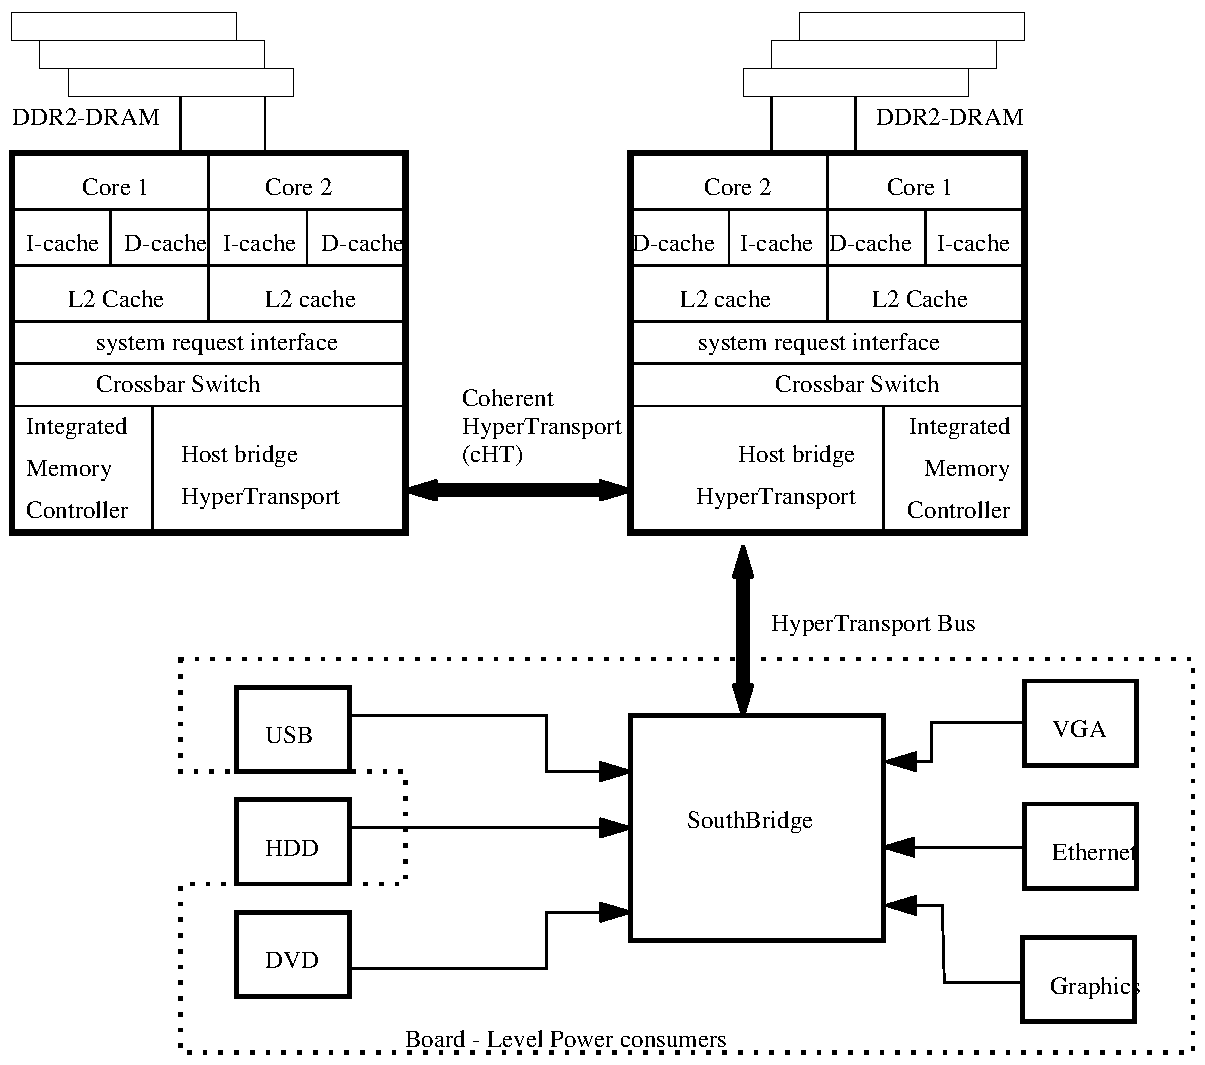
\includegraphics[scale=0.4]{x2200sys.pdf}
		\caption{Dual-core AMD Opteron based server architecture.}
		\label{fig:optarch}
	\end{center}
\end{figure}
Thus the total processor power consumption to reflect the thermal change due
to workload can be expressed as:
\begin{align}
\label{eqn:procpwr}
\bf{P_{proc}}& =  \bf{H} \cdot \bf{X}\\
& = [ \beta_0 \cdots \beta_{10} ]^T \cdot [ Var_0 \cdots Var_{10} ]^T
\end{align}
where $\bf{X}$ vector contains the following variables: ambient temperatures and
die temperatures for processors 0 and 1, HT1 and HT2 transactions, and
L2 cache misses per core.  The popularity of HyperTransport in server
and high performance computing platforms based on AMD, IBM, nVidia, Altera,
and Cray processors makes the model applicable to a wide
variety of platforms.
\subsection{DRAM Energy}
\label{sec:dram}
Energy consumed by the DRAM banks can be computed by a combination of
measuring the counts of the highest level cache miss in the processor
combined with the DRAM Read/Write power along with the DRAM background
power(activation power).  As illustrated in~\cite{Micron2007}, DRAM
background power and activation power can be obtained from the DRAM
datasheets.  For a single DRAM in our case, a total of 493mW would be
consumed. However, given the number of L2 cache misses per second when a
job is running on a certain core (over 22M / sec at the peak of bzip2
SPEC2006 benchmark), a significant amount of heat is generated from the
DRAM chips. The thermal airflow proximity of the DRAM banks to their
respective processors makes it possible for us to combine the energy
consumption and the consequent thermal output of the memory banks with the
processor ambient temperature. This value is reported by IPMI and we
combine it into our regression model.
\subsection{Hard Disk Energy}
\label{sec:hddenergy}
The energy consumed by the hard disk while operating, can be
approximated to give an upper bound on the energy consumption of the
hard disk using a combination of performance counters and drive ratings.
In our server, Hitachi's 7200 RPM, 250GB SATA hard disk~
\cite{Hitachi2006} is used.  We can achieve a crude but simple model
based on the typical power consumption data of the hard disk and
performance counters.

The utility \texttt{iostat} can be used to measure the number of read
and writes per second to the disk as well as the kilobytes read from and
written to the disk. Based on this performance counter, we can
compute an approximate disk power consumption $E_{hdd}$ value as :
\begin{align}
\label{eqn:hddpwr1}
E_{hdd}& = P_{spin-up}\times t_{su}  +  P_{read}\sum N_r\times t_r  \nonumber \\
& + P_{write}\sum N_w\times t_w + \sum P_{idle}\times t_{idle}
\end{align}
where $P_{spin-up}$ is the power required to spin-up the disk from 0 to
full rotation ($\approx 5.25$W max.). $t_{su}$ is the time required to
achieve spin up (typically about 10s). $P_{idle}$ is typically
5W. $P_{read}$ is the power consumed per kilobyte of data read from the
disk. $N_r$ is the number of kilobytes of data read in time-slice $t_r$
from the disk. $P_{read}$ and $P_{write}$ can be computed to be
approximately $13.3 \mu W$/Kbyte and $6.67 \mu W$/Kbyte.
\subsection{Electromechanical Energy}
\label{sec:electrical}
The quantity $E_{em}$ in our model takes into account the energy
consumed by the cooling fans in the server as well
as the optical drives. In our case, no performance counters are available for
the optical drive energy measurements and 
they are obtained from measurements but could easily be
obtained using current sensors at the DC output
of the power supply. Power drawn by the fans for cooling can be given
by the following equation~\cite{Bieier1997}:
\begin{equation}
\label{eq:fanp}
P_{fan}=  P_{base} \cdot \left(\frac{RPM_{fan}}{RPM_{base}} \right)^3
\end{equation}
$P_{base}$ in this case defines the base of the unloaded system. In our
system that is the power consumption of the system when running only the
base operating system and no other jobs. That value is obtained
experimentally by measuring the current drawn on the +12V and +5V lines,
using a current probe and an oscilloscope. IPMI sensors~\cite{Intel2004}
easily collect fan RPM data, and hence it is possible to quantify the
electrical power consumption in the system. Thus,
\begin{align}
\label{eqn:fanpwr}
E_{em}& = \sum P_{fan}\times t_{ipmi-slice}  + \sum P_{optical}\times t
\end{align}
\subsection{Board Components}
\label{sec:board}
The quantity $E_{board}$ captures the energy required by the support
chipsets and usually fall in the 3.3V and 5V power
domains. In our case we obtain this value using current probe based
measurements. However, as in earlier cases, current
sensors for the power lines going into the board can provide
instantaneous energy draw from the power supply. The processor,
disk, fan, and optical-drive power lines are excluded here. For our
server, at most 28 additional current sensors might be required for
the entire blade~\cite{SSI2004}. Thus:
\begin{equation}
\label{eqn:board}
E_{board} = \left(\sum V_{pow-line}\times I_{pow-line}\right) \times t_{timeslice}
\end{equation}
\subsection{Combined Model}
\label{sec:wholemodel}
The total energy consumed by the system for a given computational
workload is 
modeled as a function of these metrics as:
\begin{align}
\label{eq:linmodel}
E_{system} &=  \alpha_0 (E_{proc} + E_{mem}) + \alpha_1 E_{em} \nonumber \\
&+ \alpha_2 E_{board} + \alpha_3 E_{hdd}
\end{align}
where $\alpha_{0}$,$\alpha_{1}$,$\alpha_{2}$, and $\alpha_{3}$ are unknown
constants that are determined through linear regression analysis and
remain constant for any given server architecture.
\section{Application and Evaluation of Model}
\label{sec:experiment}
\begin{figure*}
  \begin{minipage}[b]{0.5\linewidth}
      \centering
      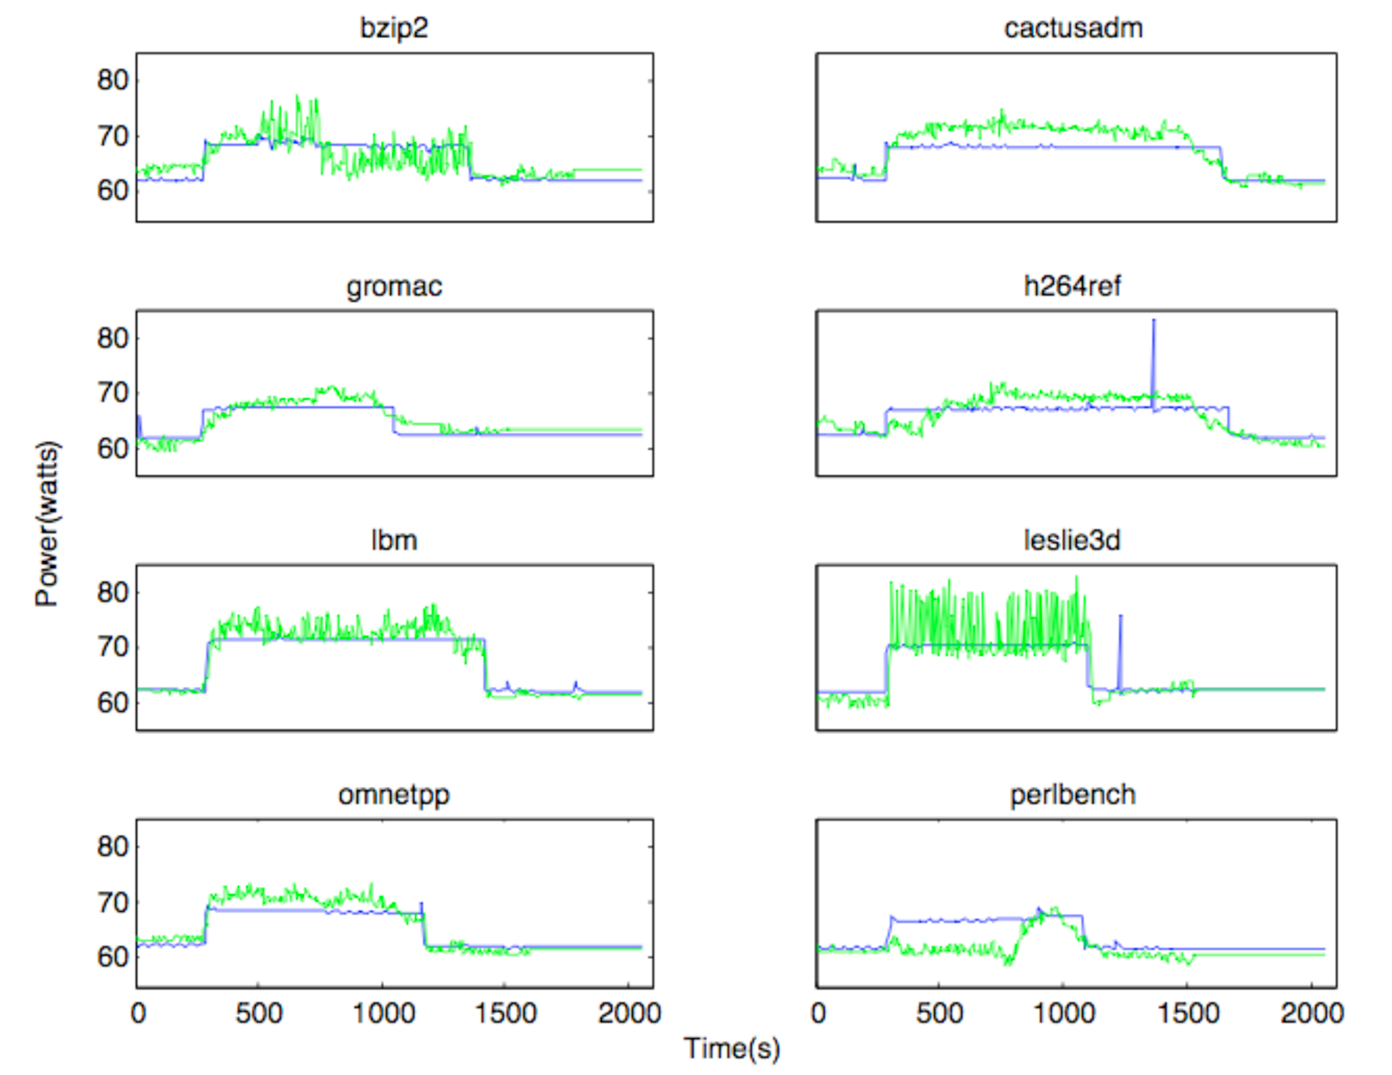
\includegraphics[width=3.4in,height=2.8in]{geomean.pdf}
      \caption{Actual vs. Predicted Power for SPEC CPU2006.}
      \label{fig:geomean}
  \end{minipage}
  \begin{minipage}[b]{0.5\linewidth}
      \centering
      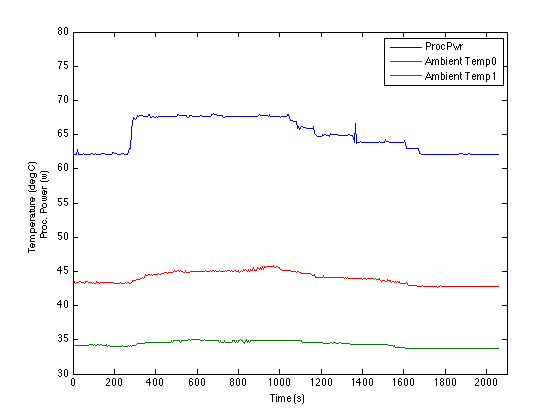
\includegraphics[width=3.4in,height=2.8in]{ppwrcputemp.png}
      \caption{Predicted Processor Power vs. CPU Temperature.}
      \label{fig:ppwrcputemp}
  \end{minipage}
\end{figure*}
The power model was calibrated to the SUT by executing eight benchmarks
from the SPEC CPU2006 benchmark suite: bzip2, cactusadm, gromac, lbm,
leslie3d, mcf, omnetpp, and perlbench~\cite{Henning2006}.  The power consumed is measured
with a WattsUP~\cite{WattsUp2006a} power meter connected between the AC
Main and System Under Test (SUT).  The internal memory of the power
meter is cleared at the start of the run and the measures collected
during the run are downloaded after the run completes from the meter's
internal memory into a spreadsheet.

Current flow on the different voltage domains in the server is measured
using an Agilent MSO6014A oscilloscope with one Agilent 1146A current
probes per system power domain (12v, 5v, and 3.3v). This data is
collected from the oscilloscope at the end of the execution of a
benchmark and stored in a spreadsheet on the test host.

Five classes of metrics are sampled at 5 second intervals during the
experiment: (1) CPU temperature for all processors in the system, (2)
Ambient temperature in the computer case measured in one more locations
using the sensors provided by server manufacturer, (3) the number of
completed transactions processed through the system bus, (4) the
number of misses that occur in the L2 cache associated with each CPU
core in the system, and (5) the amount of data transferred to/from disk.

System data is collected from the system baseboard controller using the
IPMI interface and the Solaris \texttt{iostat} utility. Processor
performance counters are collected on a system-wide basis using the
Solaris \texttt{cpustat} utility.
\begin{small}
\begin{table}[th]
  \centering
  \caption{Overall Regression Model}
  \label{tab:model}
  \begin{tabular}{c r l}
    \hline
&Coeff.&Variable\\
\hline
$\beta_{0}$& 22.80147 &\\
$\beta_{1}$&  0.73758 &Ambient Temp0\\
$\beta_{2}$&  0.00580 &Ambient Temp1\\
$\beta_{3}$&  0.00002 &CPU0 Die Temp\\
$\beta_{4}$&  0.10895 &CPU1 Die Temp\\
$\beta_{5}$&  0.00383 &HT1 Bus X-Actions\\
$\beta_{6}$&  0.00001 &HT2 Bus X-Actions\\
$\beta_{7}$&  7.36579 &L1/L2 Cache Miss for Core0\\
$\beta_{8}$&  1.18173 &L1/L2 Cache Miss for Core1\\
$\beta_{9}$&  1.18173 &L1/L2 Cache Miss for Core2\\
$\beta_{10}$& 1.38849 &L1/L2 Cache Miss for Core3\\
$\beta_{11}$& 0.00001 &Disk bytes read\\
$\beta_{12}$& 0.16657 &Disk bytes written\\
\hline \hline
  \end{tabular}
\end{table}
\end{small}

\begin{small}
\begin{table}[tbph]
  \centering
  \caption{ANOVA for Consoldated Model}
  \label{tab:anova}
  \begin{tabular}{llllll}
    \hline
    Source&~df&~~SS&~MS&~~F&P\\
    \hline
    Regr &~12&2947.92&245.66&939.56&  0.00\\
    Resid&400&~104.59&~~~0.26&&\\
    Total&412&3052.50&&\\
    \hline
    R-sq&0.97&Adj. R-sq&0.97&&\\
    \hline \hline
  \end{tabular}
\end{table}
\end{small}

The collected data was consolidated using the arithmetic mean (average)
and geometric means of the data sets.  Trial models were constructed
using each method and a statistical analysis of variance (ANOVA) was
performed to determine which model generated the best fit to the
collected data.The model was verified by examining the predicted results
for each benchmark against the data collected in the calibration test
(Fig.~\ref{fig:geomean}). A comparison between the predicted CPU power
consumption and the ambient temperatures is shown in
Fig. \ref{fig:ppwrcputemp}. The mean error per benchmark ranged from
$[1.35,2.30]$ Watts with median values in the range of $[0.83,2.40]$
watts and standard deviation between $[0.80,1.5]$ watts.

\subsection{Discussion}
\label{sec:discussions}
The consolidated model is attempting to predict for all
benchmarks. Given the large volume of data generated thorough
the different logging mechanisms, it is nearly impossible to discard bad
data.  Using the geometric mean as discussed in the previous section
helps to smooth out some of the errors introduced in the cases. However,
the diversity of the benchmarks used means that some discrepancies arise
within variables where  we expect to see tight correlations,  This, the
model predicts well in some cases and not in others.  The worst error is
no more than the four present reported above.

Also, the asymmetry of the $\beta$-coefficients for tightly correlated
variables (HT1Scaled and HT2Scaled, for example) leads us to believe
non-linear relationships may exist among these variables. Therefore,
future work needs to consider the impact of use of  non-linear
regression models together with hardware performance counters.

Another observation from the model pertains to the placement of the
temperature sensors in the server.   Ambient\_Temp0 reflects more of the
hot air flow due to the server design.   This illustrates that for
different server designs the factors controlling the thermal envelope
will be accurately reflected in the model.   Thus, we would expect to
see a more symmetric set of coefficients for Ambient\_Temp0 and
Ambient\_Temp1 had the placement of the sensors been more balanced in
the server.

In terms of measuring performance counters, we have used the Solaris 10
\texttt{cpustat}, \texttt{iostat}, and \texttt{ipmitool} utilities. Of
these, \texttt{iostat} and \texttt{ipmitool} are available across all
UNIX-based operating systems commonly used in data
centers. \texttt{cpustat} is a Solaris specific utility but is already
being ported to Linux. In future work, it is planned to use tools like
\texttt{dtrace} and \texttt{oprofile} for more controllable and tunable
performance parameters which have major impacts on system-wide and
processor wide power consumption.

The computation methodology used in this paper can be extended to other
architectures.  For example, we would measure Xeon performance counters like
\texttt{BUS\_TRANS\_ANY}, \texttt{BUS\_TRANS\_MEM}, and
\texttt{BUS\_TRANS\_BURST}.  Similar model development and coefficient
extraction arguments would hold for dual and quad core Xeons in
different processor configurations. Currently without data from the
Intel processors it is hard to say whether the model is more accurate on
a certain platform as compared to the other.

For a practical usage scenario the statistical coefficients need to be
computed only once using the SPEC benchmarks for a given server
architecture. They can be used as embedded constants available either
through the system firmware or the operating system kernel.

The model developed in this paper is valid for any AMD Opteron
dual-core/dual-processor system using the HyperTransport system
bus. However, it is scalable to any quad-core dual processors Opteron
system using HyperTransport. One would expect to see a slight difference
or variation in the predicted power due to the greater or diminished
affect of the die temperatures on the other parameters and the model
would have to be adjusted accordingly. For a dual-core quad-processor
system, the additional HT0 term would be introduced into the CPU power
consumption term and the $\beta$ coefficients would have to be
recalculated and the CPU power equation will have more terms. For a
quad-core quad processor system, similar recalculations would be
required.
\section{Conclusion}
\label{sec:conclusions}
In this paper, we have introduced a comprehensive model which uses
statistical methods to predict system-wide energy consumption  on server
blades.   The model measures energy input to the system as a function
of the work done for completing  tasks being gauged and the residual thermal
energy given off by the system as a result.   Traffic on the
system bus, misses in the L2 cache, CPU temperatures, and ambient
temperatures are combined together using linear regression techniques to
create a predictive model which can be employed to manage the processor
thermal envelope.
\begin{spacing}{0.3}
\begin{small}
\label{sec:references}
\bibliographystyle{ULieeetran}
\bibliography{hotpower08.bib}
\end{small}
\end{spacing}
\end{document}
